% IMPORTANT! In order for the document to compile, one needs to use XeLaTeX or LuaLaTeX as compiler. This can be done in  Overleaf by Menu -> Settings -> Compiler -> Choose XeLaTeX/LuaLaTeX
\documentclass[12pt]{article}

\usepackage{KUstyle}
\usepackage[margin=0.8in]{geometry} % Package for pagemargin
\usepackage{setspace} % Package for linespacing
\usepackage{tabularx} % Package for table
\usepackage{fontspec}

\setmainfont{Arial}

% This change the content of the frontpage
\ptype{[Master's thesis/Ph.d. thesis]}
\author{[Name]}
\title{[Title of thesis]}
\subtitle{[Subtitle]}
\date{Date: {[June 2021]}}
\advisor{Advisor: {[Name]}}

\renewcommand{\contentsname}{Table of content}

\begin{document}

\maketitle

\onehalfspacing

\noindent This is a template for the setup itself. The requirements for which information to include varies. You can therefore not simply use the template for your own dissertation. You can get more information about the requirements at your own study office!
\begin{table}[h]
\def\arraystretch{1.5}
\begin{tabularx}{\textwidth}{l X}
Institute: & {[Institute for Xxxxx]}  \\
Department & {[Department for Xxxxx]} \\
Author(s): & {[Name]} \\
Title and subtitle: & {[Title and subtitle of thesis]} \\
Description: & Lorem ipsum dolor sit amet, consectetur adipiscing elit. Vestibulum porttitor rhoncus dui, vehicula pellentesque odio convallis id. Vestibulum mollis nulla ut sem luctus dictum. Sed scelerisque feugiat arcu, quis faucibus lorem viverra id. Aenean dignissim metus eu ligula sagittis, at commodo magna suscipit. \\
Advisor: & {[Name]} \\
Date: & XX XX XXXX
\end{tabularx}
\end{table}
\newpage

\tableofcontents
\newpage

{\fontfamily{ptm}\selectfont


\section{Unit Roots in Danish Macro variables}



\subsection{Part 1}

\begin{figure}[h!]
    \centering
    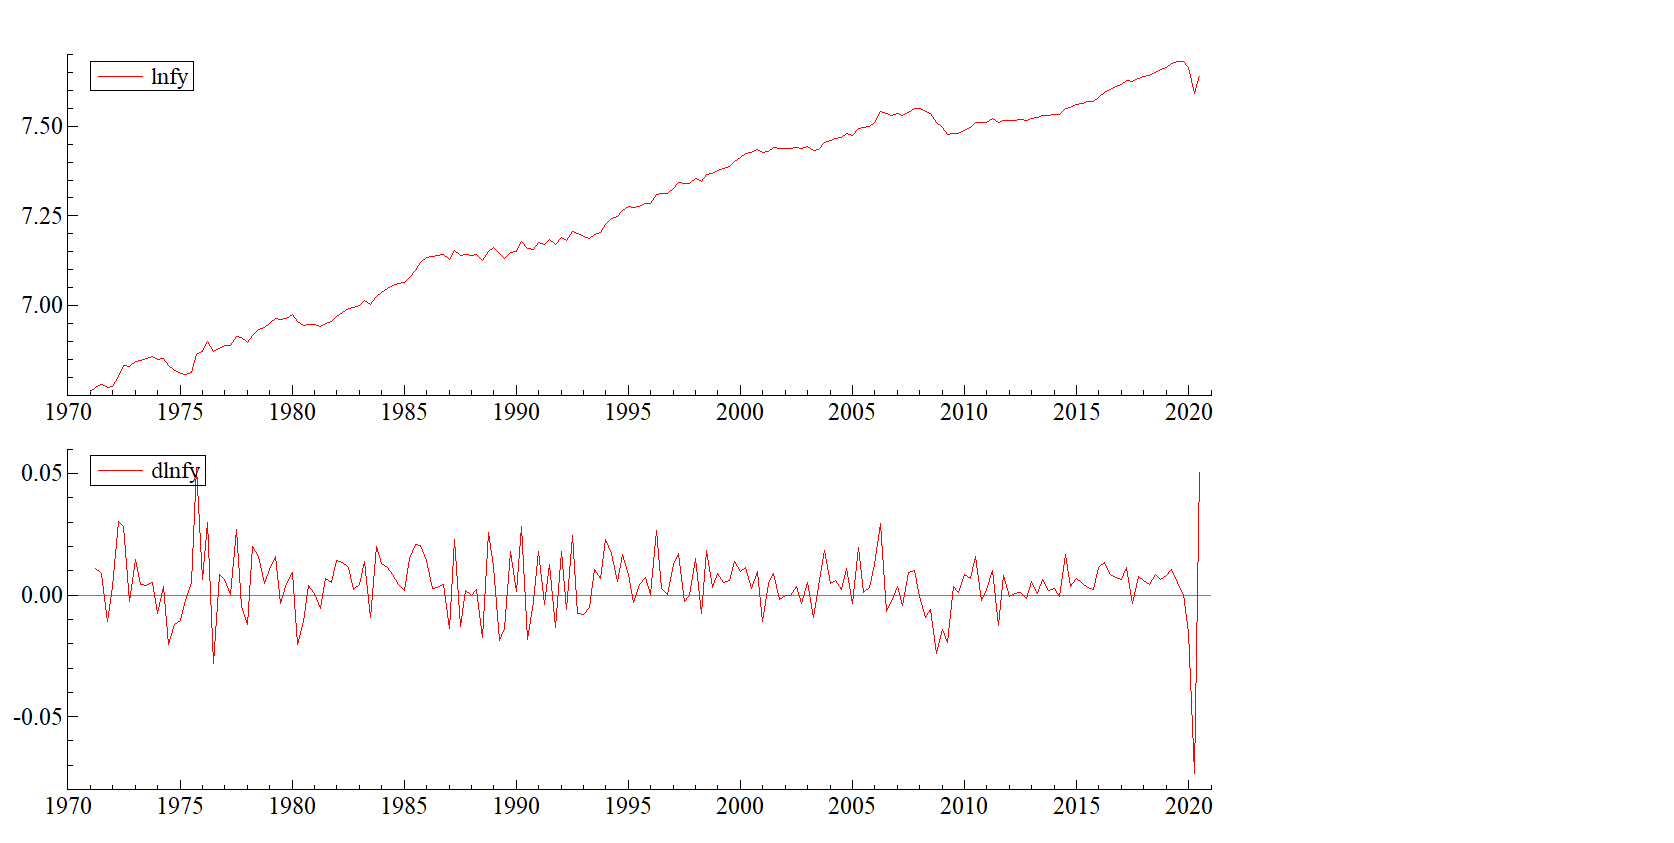
\includegraphics[scale=0.4]{Figure/fig1.png}
    \caption{Caption}
    \label{fig:my_label}
\end{figure}


\subsection{Table}

\begin{table}[tbph]
\begin{center}
\begin{tabular}{lrr}
\hline
& (1) & (2) \\
\hline
Constant & $\underset{(1.85)}{0.2871}$ & $\underset{(4.15)}{0.00435}$ \\
Trend & $\underset{(1.62)}{0.0001738}$ & . \\
dlnfy\_1 & $\underset{(-0.856)}{-0.06487}$ & $\underset{(-1.15)}{-0.08534}$ \\
dlnfy\_2 & $\underset{(1.25)}{0.1033}$ & $\underset{(1.06)}{0.08755}$ \\
lnfy\_1 & $\underset{(-1.81)}{-0.04138}$ & . \\
\hline
$\hat{\sigma}$ & 0.01295 & 0.01304 \\
Log-lik. & 576.332 & 574.051 \\
\hline
AIC & -5.830 & -5.827 \\
HQ & -5.796 & -5.807 \\
SC/BIC & -5.746 & -5.777 \\
\hline
No autocorr. 1-5 & [0.64] & [0.76] \\
No hetero. & [0.01] & [0.00] \\
Normality & [0.00] & [0.00] \\
\hline
T & 196 & 196 \\
Sample start & 1971(4) & 1971(4) \\
Sample end & 2020(3) & 2020(3) \\
\hline
\end{tabular}
\end{center}
\vspace{1em}
\caption{The table shows estimates of the model in equation (X) with various restrictions imposed. T-ratios in ($\cdot$) and p-values in [$\cdot$] for misspecification tests.}
\end{table}











}

\end{document}
